% !TEX program = pdflatex
\documentclass[conference]{IEEEtran}

\usepackage{amsmath,amssymb}
\usepackage{array}
\usepackage{booktabs}
\usepackage{cite}
\usepackage{graphicx}
\usepackage[caption=false,font=footnotesize]{subfig}
\usepackage{siunitx}
\usepackage{tabularx}
\usepackage{tikz}
\usetikzlibrary{arrows.meta,fit,positioning}
\usepackage{xcolor}
\usepackage{url}
\usepackage[hidelinks]{hyperref}

\graphicspath{{figures/}}
\sisetup{detect-all,group-separator={,},group-minimum-digits=4}
\newcommand{\method}{Adaptive DB-LBT}
\newcommand{\nru}{NR-U}
\newcolumntype{Y}{>{\raggedright\arraybackslash}X}

\hypersetup{
  pdftitle={Distributed LinUCB-Based Adaptive DB-LBT with Local Observations for Wi-Fi/NR-U Coexistence},
  pdfauthor={Yikai Wang and Yinuo Liu},
  pdfkeywords={Wi-Fi, NR-U, coexistence, listen before talk, deterministic backoff, contextual bandit}
}

\title{Distributed LinUCB-Based Adaptive DB-LBT with Local Observations\\
for Wi-Fi/NR-U Coexistence}

\author{\IEEEauthorblockN{Yikai Wang\IEEEauthorrefmark{1},
Yinuo Liu\IEEEauthorrefmark{2}}
\IEEEauthorblockA{\IEEEauthorrefmark{1}Tongji University, Shanghai, China;
2454280@tongji.edu.cn\\
\IEEEauthorrefmark{2}Shanghai Customs University, Shanghai, China;
liuyinuo@shcc.edu.cn}}

\begin{document}
\maketitle

\begin{abstract}
Deterministic backoff with listen before talk (DB-LBT) uses local countdown
interruptions to build collision-reduced Wi-Fi/NR-U access schedules. Its
recovery parameters are normally fixed, although offered load, active
contenders, and external occupancy change the backoff profile that works best.
We formulate DB-LBT parameter adaptation as a protocol-constrained contextual
bandit problem under locally observable MAC information. Each transmitter runs
LinUCB over 24 legal $(\kappa,\beta,m,b_{\mathrm{init}})$ tuples. The context
contains only local CCA, queue, delay, retransmission, and ACK/HARQ statistics;
the selected action changes the next DB-LBT recovery counter but leaves native
Wi-Fi and NR-U procedures intact.

We derive the sensing, reception, separability, and timescale conditions that
make this local context informative. Paired event experiments then compare
adaptive DB-LBT with random LBT and fixed DB-LBT. In a static $4+4$ regime,
adaptive and fixed TMC DB-LBT are numerically identical. Across held-out
scenarios, adaptation raises mean utility from $0.926467$ to $0.928023$; the
non-ideal gain is $0.289\%$. LinUCB also exceeds context-free UCB in the
combined dynamic case. A packet-level ns-3 cross-check produces mixed
technology-level directions and exposes the unresolved validation gap.

\end{abstract}

\begin{IEEEkeywords}
Wi-Fi, NR-U, coexistence, listen before talk, deterministic backoff,
contextual bandit, local observation.
\end{IEEEkeywords}

\section{Introduction}
\label{sec:introduction}

Wi-Fi and 5G New Radio in unlicensed spectrum (NR-U) contend without a common
scheduler. Both defer to detected energy and count down a backoff, yet their
surrounding procedures differ. Wi-Fi follows DCF/EDCA after an inter-frame
deferral. NR-U category-4 LBT also observes channel-occupancy limits and aligns
access to an NR transmission boundary
\cite{ieee80211_2020,3gpp37213,naik2020next}. Simultaneous counter expiry can
therefore waste airtime across both technologies.

DB-LBT replaces part of repeated random recovery with a counter derived from
locally observed countdown interruptions \cite{kosek2022dblbt}. The mechanism
can approach a collision-reduced order without node identities or
cross-technology messages. Its later TMC form remains effective under
non-full-buffer traffic, random busy periods, sensing perturbations, and
asymmetric energy detection \cite{tinnirello2026deterministic}. Those cases
also expose a control problem. A recovery tuple that admits intermittent
queues quickly can be too aggressive after more contenders become active,
whereas a conservative tuple can add avoidable delay in a light cell.

The instantaneous radio channel is not predictable from a short MAC history.
It includes nonlinear CCA threshold crossings, fading, interference, and
decoding outcomes. A transmitter nevertheless observes a slower protocol
trace: countdown freezes, queue growth, access delay, retransmissions, and
ACK/HARQ outcomes. When load or occupancy persists for several update windows,
that trace can identify which DB-LBT profile works better without reconstructing
the channel itself. This motivates our main formulation:
\emph{DB-LBT parameter adaptation is a protocol-constrained contextual bandit
under locally observable MAC information.}

The formulation targets mutually detectable indoor cells with piecewise-stable
offered load or active population. The context must be stable long enough to
learn, yet different enough across phases to make adaptation worthwhile. It is
not intended for per-packet channel prediction.

The contributions are threefold. First, we map DB-LBT recovery control to a
contextual bandit whose actions cannot alter CCA thresholds, Wi-Fi deferral,
NR-U synchronization or occupancy limits, PHY rate, or retransmission
semantics. The 24-profile design space is screened offline and reduced to two
conflicting profiles for online selection. Second, we connect the 11 local
features to protocol events and state explicit sensing, reception,
separability, and dwell-time conditions under which they are informative.
Third, a paired 32-seed experiment measures both performance and adaptation
time across repeated $4+4$ and $6+6$ phases. It finds a positive
phase-conditional effect, identifies a small high-load penalty, and preserves
the opposite whole-run diagnostic rather than hiding aggregation sensitivity.

\section{Related Work}
\label{sec:related}

Wi-Fi/NR-U coexistence schemes tune contention windows, reserve airtime,
resolve mini-slot collisions, or schedule around technology-specific timing
\cite{naik2020next,saha2021survey,kosek2021downlink}. Deterministic and
semi-random WLAN backoff instead creates post-success structure without
explicit slot assignments \cite{he2013semirandom,sanabria2017higheff}.
DB-LBT extends that idea across Wi-Fi and NR-U: interruptions estimate active
contention and set a deterministic recovery counter
\cite{kosek2022dblbt,tinnirello2026deterministic}. We retain this mechanism and
adapt only its existing recovery parameters.

Machine learning has been used throughout the IEEE 802.11 stack
\cite{szott2022wifiml}. LTE-LAA studies adapt contention windows from observed
performance \cite{ali2017ml}, and reinforcement learning can optimize
technology-level efficiency and fairness \cite{han2020rl}. Our controller has
a narrower action boundary and no shared state. LinUCB supplies uncertainty-aware
selection for a small discrete set using short local histories
\cite{li2010linucb}; the contribution is the protocol mapping and its operating
conditions, not a new bandit solver.

\section{Protocol and Local-Observation Model}
\label{sec:model}

\subsection{DB-LBT Insertion Point}

Let $\mathcal K=\mathcal K_{\rm W}\cup\mathcal K_{\rm N}$ contain the Wi-Fi
APs and NR-U gNBs sharing one channel. For local countdown slot $\ell$, node
$k$ updates
\begin{equation}
c_k(\ell+1)=
\begin{cases}
c_k(\ell)-1, & C_k(\ell)=0,\\
c_k(\ell), & C_k(\ell)=1,
\end{cases}
\label{eq:countdown}
\end{equation}
where $C_k=1$ is a busy CCA sample. A maximal busy episode freezes the
counter and increments interruption count $i_k$. In a mutually detectable
collision domain, successful peer transmissions create distinct busy episodes,
which motivates the DB-LBT estimate $\hat n_k\approx 1+i_k$.

\begin{figure}[!t]
  \centering
  \subfloat[Local observation and action boundary.]{%
    \resizebox{\columnwidth}{!}{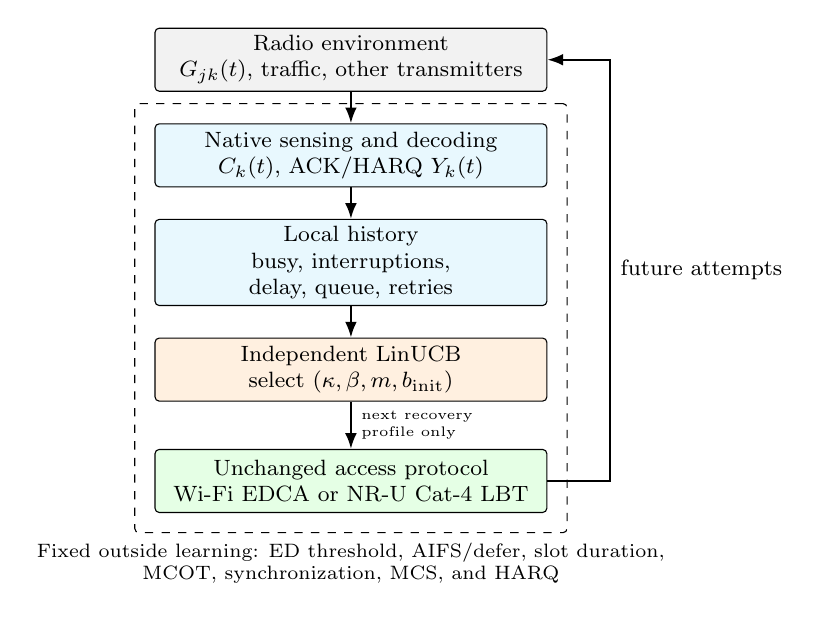
\begin{tikzpicture}[
  font=\footnotesize,
  node distance=4mm,
  block/.style={draw,rounded corners=1.5pt,align=center,minimum height=8mm,inner sep=2.5pt,text width=48mm},
  env/.style={block,fill=gray!10},
  obs/.style={block,fill=cyan!9},
  learn/.style={block,fill=orange!12},
  protocol/.style={block,fill=green!10},
  arrow/.style={-{Latex[length=2mm]},thick}
]
\node[env] (env) {Radio environment\\$G_{jk}(t)$, traffic, other transmitters};
\node[obs,below=of env] (cca) {Native sensing and decoding\\$C_k(t)$, ACK/HARQ $Y_k(t)$};
\node[obs,below=of cca] (ctx) {Local history\\busy, interruptions, delay, queue, retries};
\node[learn,below=of ctx] (agent) {Independent LinUCB\\select $(\kappa,\beta,m,b_{\rm init})$};
\node[protocol,below=6mm of agent] (mac) {Unchanged access protocol\\Wi-Fi EDCA or NR-U Cat-4 LBT};

\draw[arrow] (env) -- (cca);
\draw[arrow] (cca) -- (ctx);
\draw[arrow] (ctx) -- (agent);
\draw[arrow] (agent) -- node[midway,right=1mm,align=left,font=\tiny,
  fill=white,inner sep=0.5pt]{next recovery\\profile only} (mac);
\draw[arrow] (mac.east) -- ++(8mm,0) |- node[pos=.25,right]{future attempts} (env.east);

\node[draw,dashed,rounded corners=1.5pt,fit=(cca)(ctx)(agent)(mac),inner sep=2.5mm,
  label={[align=center,font=\scriptsize]below:{Fixed outside learning: ED threshold, AIFS/defer, slot duration,\\MCOT, synchronization, MCS, and HARQ}}] {};
\end{tikzpicture}
}}\\[-1mm]
  \subfloat[Insertion point in Wi-Fi and NR-U access.]{%
    \resizebox{\columnwidth}{!}{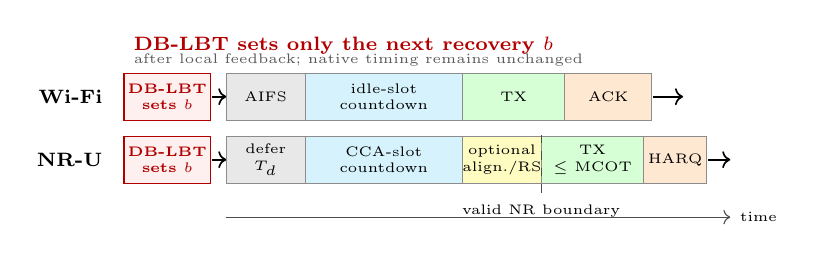
\begin{tikzpicture}[font=\scriptsize,x=1mm,y=1mm]
\tikzset{
  phase/.style={draw=black!45,minimum height=6mm,inner sep=0pt,
    align=center,text=black,font=\tiny},
  learned/.style={phase,draw=red!70!black,fill=red!6,
    text=red!70!black,font=\tiny\bfseries},
  native/.style={phase,fill=gray!18},
  countdown/.style={phase,fill=cyan!16},
  transmit/.style={phase,fill=green!16},
  feedback/.style={phase,fill=orange!18},
  alignment/.style={phase,fill=yellow!24}
}

\node[anchor=west,text=red!70!black,font=\scriptsize\bfseries]
  at (10,18.5) {DB-LBT sets only the next recovery $b$};
\node[anchor=west,text=black!65,font=\tiny]
  at (10,16.7) {after local feedback; native timing remains unchanged};

\node[anchor=east,font=\scriptsize\bfseries] at (8.5,12) {Wi-Fi};
\node[learned,minimum width=11mm] at (15.5,12) {DB-LBT\\sets $b$};
\draw[->,semithick] (21.2,12) -- (23,12);
\node[native,minimum width=10mm] at (28,12) {AIFS};
\node[countdown,minimum width=20mm] at (43,12) {idle-slot\\countdown};
\node[transmit,minimum width=13mm] at (59.5,12) {TX};
\node[feedback,minimum width=11mm] at (71.5,12) {ACK};
\draw[->,semithick] (77.2,12) -- (81,12);

\node[anchor=east,font=\scriptsize\bfseries] at (8.5,4) {NR-U};
\node[learned,minimum width=11mm] at (15.5,4) {DB-LBT\\sets $b$};
\draw[->,semithick] (21.2,4) -- (23,4);
\node[native,minimum width=10mm] at (28,4) {defer\\$T_d$};
\node[countdown,minimum width=20mm] at (43,4) {CCA-slot\\countdown};
\node[alignment,minimum width=10mm] at (58,4) {optional\\align./RS};
\node[transmit,minimum width=13mm] at (69.5,4) {TX\\$\leq$ MCOT};
\node[feedback,minimum width=8mm] at (80,4) {HARQ};
\draw[->,semithick] (84.2,4) -- (87,4);

\draw[dashed,black!70] (63,-0.2) -- (63,7.2);
\node[anchor=north,align=center,text=black,font=\tiny] at (63,-0.5)
  {valid NR boundary};
\draw[->,black!70] (23,-3.3) -- (87,-3.3)
  node[anchor=west,text=black,font=\tiny] {time};
\end{tikzpicture}
}}
  \caption{Each transmitter selects only its next DB-LBT recovery profile.
  Native CCA, countdown, synchronization, MCOT, and ACK/HARQ behavior remain
  outside the learner.}
  \label{fig:protocol}
\end{figure}

Figure~\ref{fig:protocol} locates the control boundary. DB-LBT supplies the
next recovery counter after an ACK/HARQ outcome. Wi-Fi still applies its
inter-frame deferral and EDCA rules; NR-U still applies its priority class,
maximum channel occupancy, and transmission-boundary alignment
\cite{kosek2021downlink,3gpp37213}.

\subsection{What Local History Can Represent}

Propagation gain $G_{jk}(t)$ includes path loss, shadowing, and small-scale
fading. CCA and reception compress that nonlinear channel into protocol
outcomes:
\begin{align}
C_k(t)&=\mathbb 1\!\left\{N_k+\sum_{j\ne k}a_j(t)P_jG_{jk}(t)
\geq\Gamma_k\right\},
\label{eq:cca}\\
\Pr\{Y_k=1\mid\gamma_k,u_k\}
&=1-\mathrm{PER}_{\tau_k}(\gamma_k,u_k).
\label{eq:success}
\end{align}
A failed packet can thus result from simultaneous access, fading, hidden
interference, or decoding. The learner never treats one failure as a collision
measurement.

Three conditions connect these outcomes to the event-level contention model:
(A1) every co-channel transmission exceeds every contender's CCA threshold;
(A2) isolated reception succeeds with high probability; and (A3) simultaneous
transmissions have no capture. Then
\begin{equation}
\begin{aligned}
C_k(\ell)&=\mathbb 1\!\left\{\sum_{j\ne k}a_j(\ell)>0\right\},\\
Y_k(\ell)&=1\iff\sum_j a_j(\ell)=1.
\end{aligned}
\label{eq:reduction}
\end{equation}
Busy episodes now carry contention information: one zero counter succeeds and
multiple zeros collide. Equation~\eqref{eq:reduction} is an abstraction for
the event experiment, not a claim that a fading PHY is linear.

The controller aggregates 11 measurements already available at an AP or gNB:
success and failure ratios, CCA busy fraction, countdown interruptions, delay
EWMA and P95, queue occupancy, arrivals, retransmissions, effective-data
occupancy, and $\hat n_k=\operatorname{clip}(1+\bar i_k,1,32)$. CCA and
interruptions indicate occupancy; queue and delay reveal demand; ACK/HARQ and
retransmissions describe service after access. Periodic occupancy or a changed
active set need not be explicitly labeled if it leaves a distinct local trace.

\begin{table}[!t]
\caption{Local Features and Their Protocol Origin}
\label{tab:context}
\centering
\scriptsize
\begin{tabularx}{\columnwidth}{@{}p{19mm}p{24mm}Y@{}}
\toprule
Feature group & Local source & Action-relevant cue \\
\midrule
Busy fraction, interruptions & CCA and countdown freezes & Active peers or persistent occupancy \\
Success, failure, retries & ACK/HARQ and retry state & Service after attempted access \\
Queue, arrivals, delay & Local traffic and MAC queue & Activation and congestion \\
Effective-data occupancy, busy share & Successful channel use & Schedule efficiency and local share \\
\bottomrule
\end{tabularx}
\end{table}

Let $z$ denote a MAC occupancy regime, $q^\star(z)$ its best allowed profile,
and $\bar x_k(z)$ node $k$'s mean context. Action-relevant local separability
requires
\begin{equation}
q^\star(z)\ne q^\star(z')\Longrightarrow
\|\bar x_k(z)-\bar x_k(z')\|_2\geq\delta_x>0.
\label{eq:identifiability}
\end{equation}
The corresponding timescales are
\begin{equation}
T_{\rm phy}\ll T_{\rm ctx}\lesssim T_{\rm adapt}
\ll T_{\rm dwell}<T_{\rm hor}.
\label{eq:timescale}
\end{equation}
Fast radio and arrival randomness can then average into history before a phase
changes, while at least one change occurs within the operating horizon.
Equations~\eqref{eq:identifiability}--\eqref{eq:timescale} define the difficult
but testable setting in which local adaptation is useful.

\section{Protocol-Constrained Contextual Bandit}
\label{sec:method}

\subsection{Legal DB-LBT Actions}

After queue activation, node $k$ draws
$b_k\sim\mathcal U[0,b_{\mathrm{init}}]$. Once an attempt completes, DB-LBT
sets the recovery counter
\begin{equation}
b_k^{+}=
\begin{cases}
\alpha+i_k, & r_k\bmod\kappa<\beta,\\
\mathcal U[0,m], & \text{otherwise},
\end{cases}
\label{eq:dblbt}
\end{equation}
where $r_k$ is the retransmission count. The deterministic branch turns
interruptions into schedule spacing; the short random branch separates
coincident schedules. We retain $\alpha=11$ and expose only the four recovery
parameters in Table~\ref{tab:mapping}.

\begin{table}[!t]
\caption{Contextual-Bandit Actions and Protocol Meaning}
\label{tab:mapping}
\centering
\footnotesize
\begin{tabularx}{\columnwidth}{@{}c p{15mm}Y@{}}
\toprule
Variable & Values & DB-LBT role \\
\midrule
$\kappa$ & $5,7$ & Recovery-cycle length indexed by retransmissions. \\
$\beta$ & $2,3$ & Early states using interruption-derived spacing. \\
$m$ & $4,6,10$ & Maximum random backoff after repeated failure. \\
$b_{\rm init}$ & $15,31$ & Initial range when a queue becomes active. \\
\midrule
$\alpha$ & fixed 11 & Common idle-space offset. \\
\bottomrule
\end{tabularx}
\end{table}

The Cartesian product contains 24 arms and always satisfies
$\beta<\kappa$. It is centered on the published TMC tuple
$(7,3,6,15)$: $b_{\rm init}=15$ matches the common minimum contention
window, 31 gives a more conservative activation range, and each $m$ is below
$\alpha$. An action supplies only the next counter. CCA thresholds,
AIFS/defer timing, NR-U priority class and MCOT, synchronization, MCS, and
ACK/HARQ processing stay fixed by the technology and scenario.

Each parameter addresses a distinct recovery moment. The activation range
$b_{\rm init}$ controls how aggressively a newly nonempty queue enters an
existing schedule. Parameters $\kappa$ and $\beta$ determine how often early
retransmission states return to interruption-derived spacing, while $m$
controls the random escape after repeated failure. A larger value is not
uniformly better: conservative activation can avoid a burst collision but
adds delay when few nodes are active, and extra random recovery can separate
colliding schedules while weakening deterministic reuse. This tradeoff is the
reason to select complete tuples rather than tune one scalar.

\subsection{Local LinUCB Controller}

Each node retains at most 64 of its own attempts. Its 11-dimensional context
$x_k$ contains success/failure ratios, CCA busy fraction, countdown
interruptions, delay EWMA and P95, queue occupancy, arrivals, retransmissions,
effective-data occupancy, and
$\hat n_k=\operatorname{clip}(1+\bar i_k,1,32)$. No peer identity, peer queue,
global fairness value, or cross-technology message enters the vector.

The action space is discrete, the context is low dimensional, and online
samples are scarce. LinUCB fits this setting with one linear reward model per
arm and an explicit exploration bonus. Within a locally separable regime, the
working approximation is
\begin{equation}
\mathbb E[R_{k,t}\mid x_{k,t}=x,q_{k,t}=q,z]
\simeq x^{\mathsf T}\theta_{k,q}^{(z)}.
\label{eq:linear-reward}
\end{equation}
The model is linear in context within one arm; it is not linear in the four
DB-LBT parameters. Keeping a separate $\theta_{k,q}^{(z)}$ for every tuple
allows parameter interactions to differ across arms. It also avoids imposing a
monotone ordering on $\kappa$, $\beta$, $m$, or $b_{\rm init}$. Thus the
nonlinear CCA and decoding maps in \eqref{eq:cca}--\eqref{eq:success} remain
outside the learner, while the locally observed reward surface is approximated
where decisions are actually made.

For each arm $q$, the controller maintains
$A_q\in\mathbb R^{11\times11}$ and $d_q\in\mathbb R^{11}$:
\begin{align}
\hat\theta_q&=A_q^{-1}d_q,\\
p_q(x_k)&=\hat\theta_q^{\mathsf T}x_k+
c\sqrt{x_k^{\mathsf T}A_q^{-1}x_k},\\
q^*&=\arg\max_q p_q(x_k),
\label{eq:linucb}
\end{align}
with $c=0.5$. After observing reward $R_k$, the selected model receives
$A_q\leftarrow A_q+x_kx_k^{\mathsf T}$ and
$d_q\leftarrow d_q+R_kx_k$.

The reward is local as well. Let $A_k$ be effective-airtime fraction,
$D_{95,k}$ P95 delay, $s_k$ the node's successful-busy share, and $P_{f,k}$ its
failure ratio:
\begin{align}
U_A&=\operatorname{clip}(\hat n_kA_k,0,1),\\
U_D&=1-\operatorname{clip}
 \left(\frac{D_{95,k}}{16\,\mathrm{ms}\,\hat n_k},0,1\right),\\
U_S&=1-\operatorname{clip}
 \left(\frac{|s_k-1/\hat n_k|}{1/\hat n_k},0,1\right),\\
R_k&=(U_A+U_D+U_S)/3-0.25P_{f,k}.
\label{eq:reward}
\end{align}
Every transmitter owns a controller initialized from the same offline model.
After eight observations, the event implementation decides every 32 global
contention rounds; the packet implementation decides every 32 completed local
attempts. A decision affects the next recovery only, never a countdown already
in progress.

\subsection{Initialization and Online Sequence}

Offline initialization evaluates every arm under 11 topology, load,
interference, and sensing conditions using three training seeds. Those samples
populate the 24 linear models before formal evaluation; none of the ten formal
event seeds is used for initialization or fixed-oracle selection. The same
initial model is copied to each transmitter, but subsequent contexts, choices,
rewards, and updates are local.

An online step follows the protocol clock. The node first aggregates its latest
history into $x_k$, selects $q^*$ with \eqref{eq:linucb}, and applies that tuple
only when the current attempt has completed. It then observes the next reward
window and updates the chosen arm. Separating observation, selection,
application, and reward assignment prevents an action from receiving credit
for a countdown that began under an earlier profile.

\section{Evaluation}
\label{sec:evaluation}

\subsection{Paired Phase Experiment}

The event simulator implements the contention reduction in
\eqref{eq:reduction}. A transmission occupies \SI{2}{\milli\second}; Wi-Fi and
NR-U use equal contention windows $[15,63]$, and NR-U access is aligned to a
\SI{250}{\micro\second} grid. Exogenous arrival and contention streams are
paired between Adaptive DB-LBT and fixed TMC. The 32 formal seeds, ranging
from 20029 to 20341, were frozen before the pilot and do not overlap the three
discovery seeds.

Each 32,768-round run alternates two 4096-round phases four times. The light
phase activates four Wi-Fi and four NR-U nodes with Poisson rate 0.025
packets/ms per node. The high phase activates all six nodes of each technology
at rate 0.045. Thus each seed contains seven observed transitions and equal
dwell time in both regimes.

\begin{table}[!t]
\caption{Formal Confirmation Design}
\label{tab:formal-design}
\centering
\footnotesize
\begin{tabularx}{\columnwidth}{@{}p{25mm}Y@{}}
\toprule
Item & Frozen value \\
\midrule
Compared policies & Distributed LinUCB over $q_4/q_{20}$; fixed $q_{20}$ TMC \\
Formal evidence & 32 paired seeds; discovery seeds excluded \\
Light phase & $4+4$, Poisson 0.025 packets/ms/node \\
High phase & $6+6$, Poisson 0.045 packets/ms/node \\
Schedule & Eight 4096-round phases; 32,768 rounds/run \\
Inference & Seed-paired bootstrap, 10,000 resamples \\
\bottomrule
\end{tabularx}
\end{table}

The reporting utility is separate from the local reward in
\eqref{eq:reward}:
\begin{align}
U_D^{\rm eval}&=1-\operatorname{clip}(D_{95}/500\,\mathrm{ms},0,1),\nonumber\\
U_{\rm eval}&=(A_{\rm total}+U_D^{\rm eval}+J)/3-0.25P_{\rm col}.
\label{eq:evaluation-utility}
\end{align}
It combines effective data airtime, P95 access delay, Jain fairness, and event
collision probability. We first recompute all four components within every
contiguous phase, average the eight phase utilities within a seed, and form
paired bootstrap intervals across seeds. This phase-conditional estimand keeps
the active population fixed inside each metric calculation.

\begin{figure*}[!t]
  \centering
  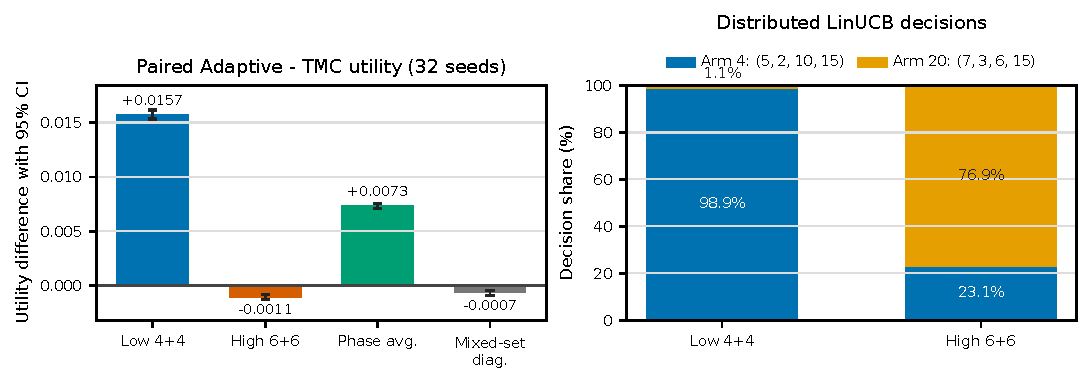
\includegraphics[width=.96\textwidth]{restricted-confirmation.pdf}
  \caption{Independent 32-seed confirmation. Left: Adaptive-minus-TMC utility;
  intervals are paired 95\% bootstrap CIs. ``Phase avg.'' is the primary
  within-phase estimator, while ``Mixed-set diag.'' computes one utility over
  the entire run. Right: online choices are restricted to the two profiles in
  Table~\ref{tab:profiles}.}
  \label{fig:restricted}
\end{figure*}

\subsection{Performance and Decisions}

Figure~\ref{fig:restricted} shows a strong regime split. In the light $4+4$
phase, Adaptive DB-LBT improves utility by $0.015735$ (95\% CI
$[0.015322,0.016145]$), and all 32 seed differences are positive. In the high
$6+6$ phase the effect is $-0.001058$
($[-0.001283,-0.000843]$); only one seed is positive. Averaging equal-duration
phases gives $+0.007338$ ($[0.007093,0.007584]$), positive for every seed.

The component differences explain that result. Relative to TMC, the
phase-averaged collision probability falls by 0.032288 and Jain fairness rises
by 0.000245. Effective airtime falls by 0.002059, while P95 delay increases by
\SI{193.3}{\micro\second}. The utility gain is therefore a collision reduction
that outweighs small airtime and delay costs; it is not a uniform improvement
of every metric.

Arm choices follow the offline conflict. Nodes choose $q_4$ for 98.9\% of
light-phase decisions. In the high phase, the fixed-TMC profile $q_{20}$ rises
to 76.9\%. Residual exploration of $q_4$ is consistent with the small high-load
penalty. This behavior also gives a protocol interpretation to the light-load
gain: queues repeatedly enter contention, and the shorter recovery cycle with
$m=10$ is favored; persistent high load returns most decisions to TMC.

We measure adaptation from the local reward trace after every explicit phase
change. Recovery is the first of three consecutive eight-decision windows that
reaches 90\% of the improvement from the immediate post-change level to the
last-quarter phase level. All 224 transitions recover without censoring.
Median $T_{\rm adapt}$ is 736 rounds and the 95th percentile is 928 rounds,
well below $T_{\rm dwell}=4096$. The experiment therefore checks, rather than
only assumes, the critical ordering in \eqref{eq:timescale} for this scenario.

\subsection{Aggregation Sensitivity and Packet Check}

A whole-run calculation pools phases before forming the nonlinear utility.
It gives $-0.000668$ ($[-0.000921,-0.000413]$), with 6/32 positive seeds.
The direction changes because the active population, delay distribution, and
fairness denominator are mixed before normalization; the corresponding
airtime, P95-delay, and fairness differences become $-0.013570$,
$+\SI{2.240}{\milli\second}$, and $-0.008170$. We retain this diagnostic because
an application that values one end-to-end mixed-population score should not
substitute the phase-conditional conclusion.

The repository also contains an ns-3.35/5G-LENA/NR-U protocol cross-check with
Wi-Fi EDCA, NR-U alignment, HARQ, and a frequency-selective channel. That older
three-seed campaign used the initial unrestricted 24-profile model, so its
mixed technology-level directions are not treated as confirmation of the
restricted controller.

\begin{table}[!t]
\caption{Five-Second ns-3 Shadowing Diagnostic (TMC, Seed 410)}
\label{tab:ns3-diagnostic}
\centering
\scriptsize
\begin{tabular}{@{}lrrrr@{}}
\toprule
Tech. & Thr. (Mb/s) & Delay (ms) & IP loss & Access overlap \\
\midrule
Wi-Fi & 8.121 & 1.793 & 0.0117 & 0.3093 \\
NR-U  & 7.537 & 38.087 & 0.0828 & 0.7726 \\
\bottomrule
\end{tabular}
\end{table}

Table~\ref{tab:ns3-diagnostic} is a measurement-path diagnostic with 3GPP
shadowing enabled, not an adaptive-policy comparison. The access quantity is
the fraction of transmission starts overlapping another active transmission;
IP loss is computed from transmitted and received packets. Their different
values confirm that decoding loss and simultaneous access must remain separate.

\section{Discussion}
\label{sec:discussion}

\subsection{Why a Linear Contextual Model Is Enough}

The learner does not predict a waveform or an instantaneous channel gain.
Native CCA and ACK/HARQ processing have already converted those quantities into
busy periods, interruptions, successes, and delays. For the controller, the
relevant surface is the reward difference among 24 legal recovery profiles.
An 11-dimensional linear model is a useful first approximation to that small
surface, and LinUCB adds directed exploration when online samples are limited.
The UCB ablation supports the value of context; the unresolved feature
ablations do not motivate a larger nonlinear model.

The scenario differences also fit the protocol interpretation. Under light
Poisson traffic, queues repeatedly enter and leave contention, so activation
and recent service history can distinguish useful profiles. Heavy Poisson
traffic behaves more like a persistently active set, where fixed TMC is already
strong and exploration can cost utility. The combined case mixes arrivals,
periodic occupancy, and active-set turnover; there, contextual LinUCB separates
from UCB even though no single feature-group removal is decisive. These
patterns explain the aggregate gain without suggesting that adaptation should
improve every load.

\subsection{Distributed-Learner Interpretation}

When several nodes adapt, node $k$ receives reward
$R_k(\boldsymbol q_t)$ under the joint arm vector
$\boldsymbol q_t=(q_{1,t},\ldots,q_{|\mathcal K|,t})$. This interaction may be
read as a restricted stochastic contextual bandit game. The reading is valid
when peer actions are non-anticipating within the current decision interval,
their joint policy changes little over $T_{\rm adapt}$, and updates are
asynchronous or weakly coupled. Peers may learn under those conditions because
their aggregate behavior changes slowly enough over a local update
window. Rapid synchronized co-adaptation, action-conditioned retaliation, or
jamming breaks that approximation. The interpretation supplies neither a Nash
convergence result nor an adversarial-regret guarantee.

\subsection{Limitations and Future Work}

The operating region lies between two unhelpful extremes. A fixed occupancy
process needs no adaptation; a process that changes faster than context can be
collected makes history stale. Equation~\eqref{eq:timescale} instead assumes
locally distinguishable phases with enough dwell time for learning. Separate
Poisson-rate runs establish load dependence, while the event
\texttt{dynamic-combined-4x4} case is a faster stress test: nodes join every
10 global rounds, stay active for 200 rounds, and decisions occur every 32 rounds.
Neither experiment directly estimates $T_{\rm adapt}$.

Physical validation is also incomplete. The ns-3 runs use fixed positions,
disabled log-normal shadowing, one static frequency-selective channel draw, and
only three two-second seeds. A stronger study should separate propagation and
decoding measurements (SINR, PER/BLER, MCS, coherence time) from sensing
measurements (energy-detection margin and miss/false-busy rates). MAC service
needs simultaneous-access collisions, airtime, retransmissions, and delay
tails; learning dynamics needs recovery time and performance versus
$T_{\rm adapt}/T_{\rm dwell}$. These four measurement classes would show whether a
sliding-window learner, change-point reset, or nonlinear reward model is
actually warranted.

\section{Conclusion}
\label{sec:conclusion}

We cast DB-LBT recovery adaptation as a protocol-constrained contextual bandit
driven by local MAC history. Offline screening reduces 24 legal tuples to two
profiles with opposite light/high-load rankings; distributed LinUCB then
selects between them without shared state or changes to native Wi-Fi and NR-U
procedures. In the tested phase-conditional setting, the method improves
utility for all 32 formal seeds and recovers well before the next regime
change. Its high-load penalty and negative whole-run diagnostic define the
boundary of that conclusion as clearly as the light-load gain.


\section*{Appendix}
The complete reproducibility package, including source code, configurations,
seeds, results, and figures, is available at:
\begin{center}
\url{https://github.com/Ignister01/distributed-linucb-dblbt}
\end{center}

\IEEEtriggeratref{4}
\bibliographystyle{IEEEtran}
\bibliography{references}

\end{document}
